\newchapter{feedforward}{Feedforward Results}

This is the introductory text.

\newsection{gainScans}{Gain Scans}

\newsection{jitterRecord}{Lowest Achieved Phase Jitter}

The results presented in this section show the best downstream phase jitter currently achieved at CTF3 with the PFF correction. The dataset was taken on Friday 20th November 2015 at 15:38 and comprises 172 pulses taken in interleaved mode, with the correction applied to the 86 even indexed pulses and no correction applied to the remaining 86 odd indexed pulses. Naturally, this dataset was taken during the best beam conditions currently achieved at CTF3 in terms of phase propagation, taken just after a series of R56 and beam energy optimisations using the same methods discussed in Chapter \ref{c:phasePropagation}.

\begin{figure}
  \centering
  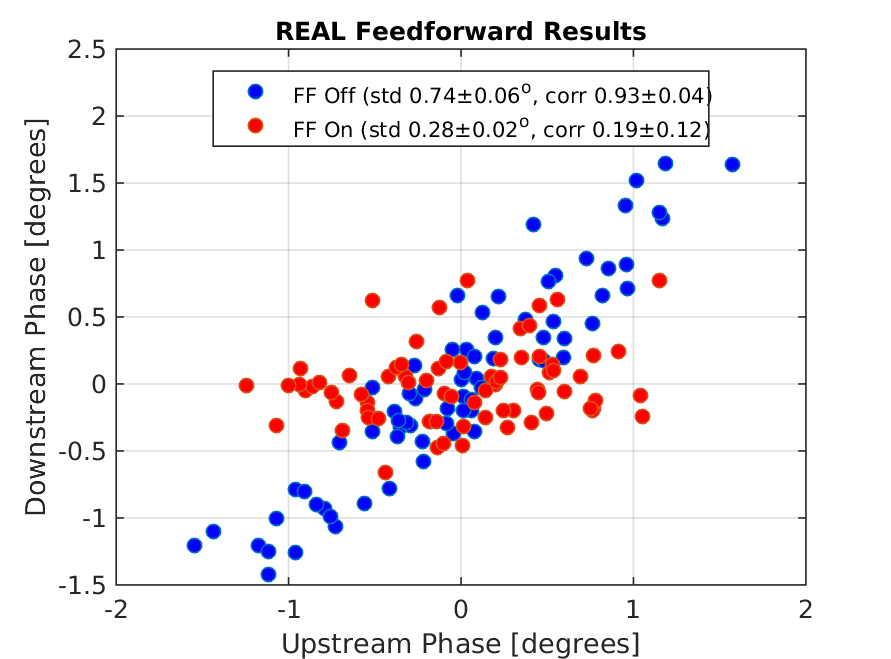
\includegraphics[width=0.45\textwidth]{Figures/BestFF_Real}
  \caption{Mean phase.}
  \label{f:BestFF_Real}
\end{figure}

\begin{figure}
  \centering
  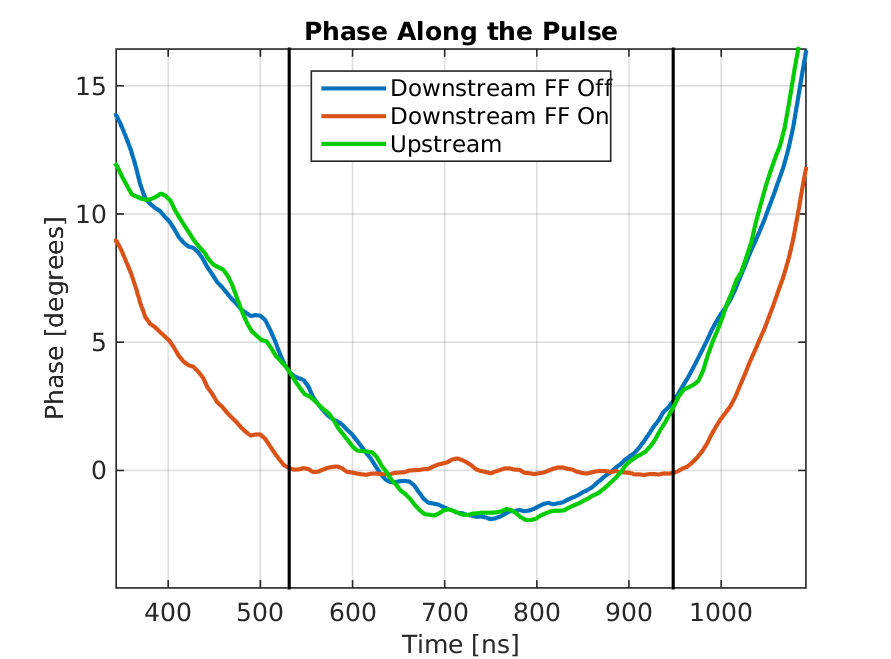
\includegraphics[width=0.45\textwidth]{Figures/BestFF_MeanPhaseAlong}
  \caption{Mean phase along.}
  \label{f:BestFF_MeanPhaseAlong}
\end{figure}

\begin{figure}
  \centering
  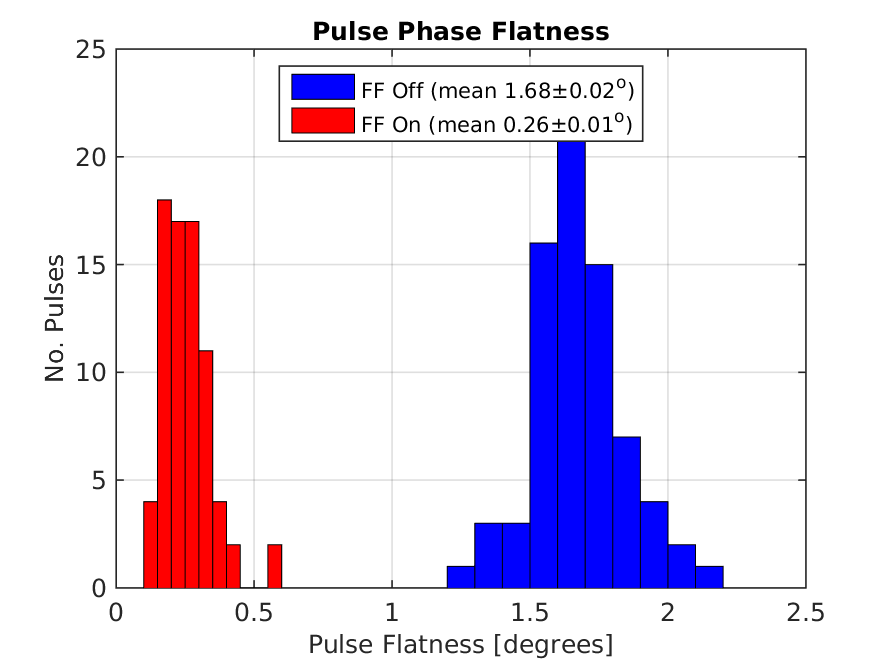
\includegraphics[width=0.45\textwidth]{Figures/BestFF_Flatness}
  \caption{Flatness.}
  \label{f:BestFF_Flatness}
\end{figure}

\newsection{s:simFF}{Simulated PFF Results}

\begin{figure}
  \centering
  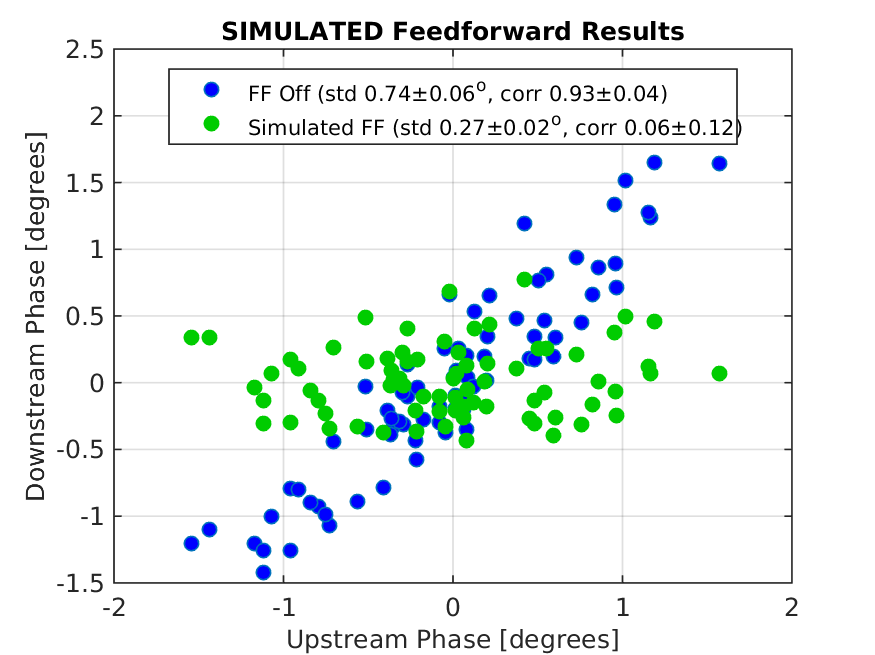
\includegraphics[width=0.45\textwidth]{Figures/BestFF_Simulated}
  \caption{Simulated PFF.}
  \label{f:BestFF_Simulated}
\end{figure}

\newsection{longPFF}{Correction on Longer Timescales}

\newsection{pffNovelSetups}{Correction with Additional Jitter Source}

\newsection{slowCorr}{Slow Correction}

\subsection{Implementation}
\label{ss:slowCorrMethod}

\subsection{Results}
\label{ss:slowCorrResults}




